\section{Summary of Papers}
\label{sec:summary}

\subsection{AutoNER}
AutoNER \cite{autoner} has two contributions: Fuzzy LSTM CRF and Tie-or-Break scheme.
\\

\noindent\textbf{Fuzzy LSTM CRF}
Have to read about CRF and how they work. 
\begin{enumerate}
	\item Neither BERT nor ELMO use CRF and both report SOTA results on NER.
	\item Need to check if CRFs work for domain specific case? If so, why?
\end{enumerate}

They also introduce a training mechanism which models the noise in supervision. \\



\noindent\textbf{Tie-or-Break Scheme}
In a sentence, predict whether two words should be tied together to form one phrase or broken apart. Now, between every to 'breaks' you have a potential named entity. Predict its type ('None' being the type that it's not a named entity).

Training data for these phrases comes from another paper of the same group \cite{autophrase} which uses unsupervised methods to extract interesting phrases from a large corpus.
\\

\begin{figure*}[h!]
	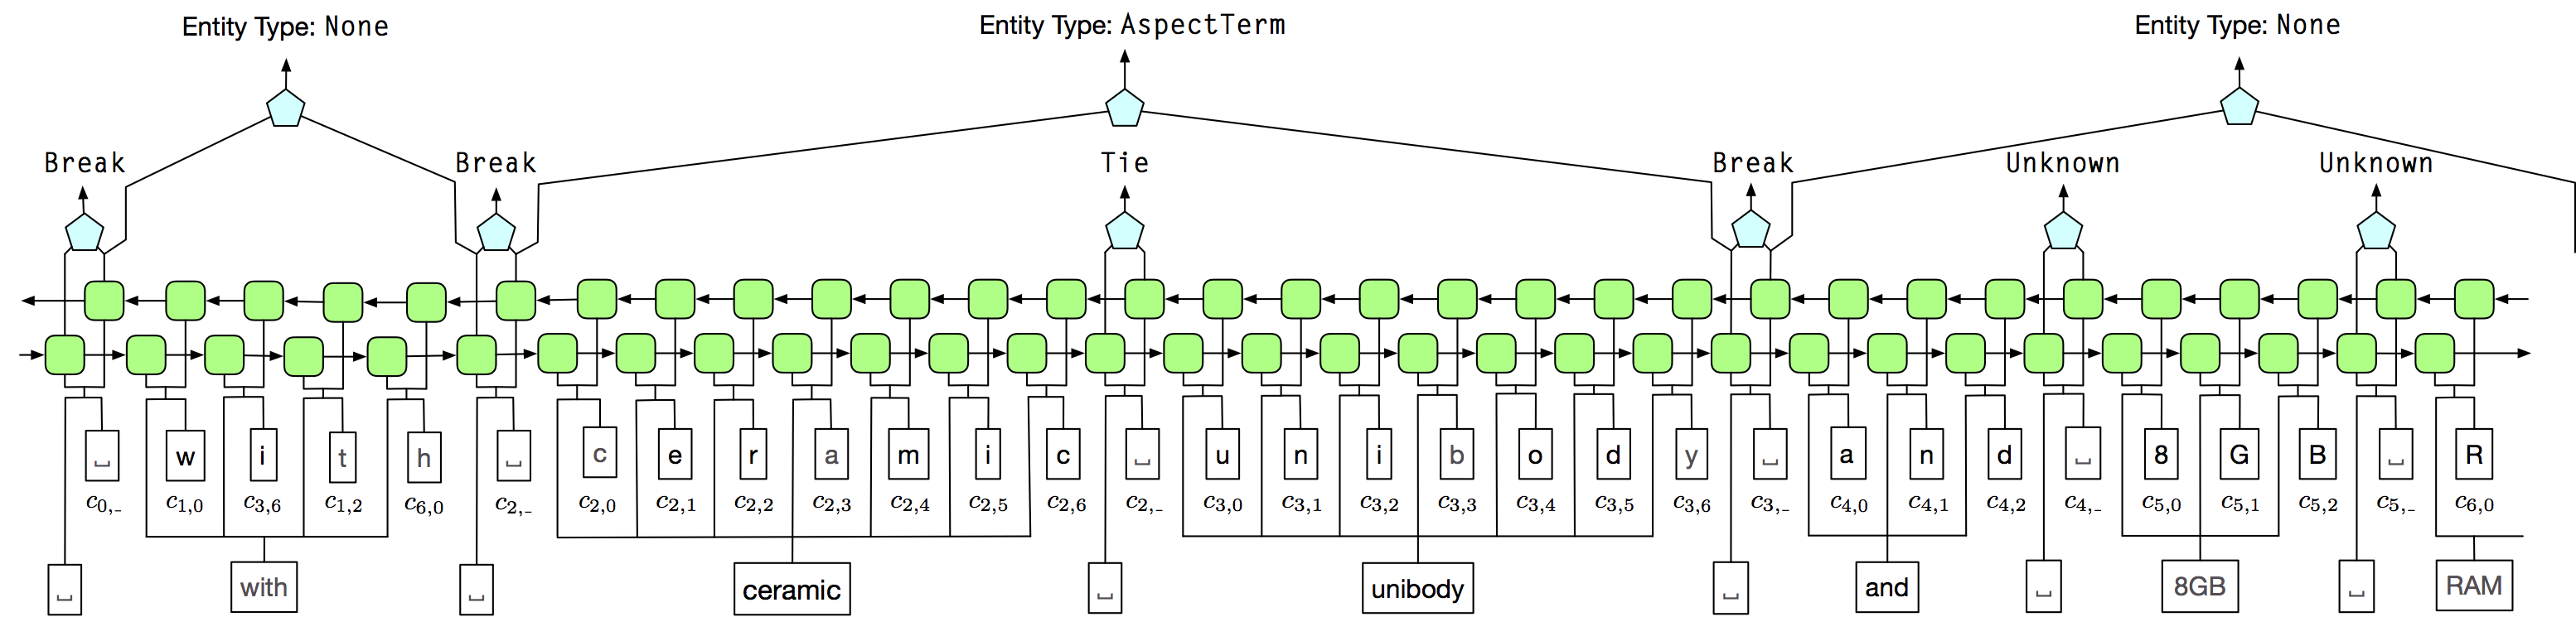
\includegraphics[scale=0.3]{images/autoner_tie_or_break.png}
	\caption{\label{fig:tie_or_break}Overview of the Tie-or-Break scheme used in AutoNER.}
\end{figure*}

\subsection{Character Level Language Modeling}
\begin{enumerate}
	\item Character level features are important for NER. For instance, first letter being capitalized implies a proper noun, names of places in North India typically end in '-pur' (like Jaipur, Raipur) etc.
	\item For char-level LM, sequence lengths become too large to be directly fed into a Transformer Network. Naive solution is to break a sequence down into shorter pieces but then you lose context. One way to retain context is to keep a \textit{memory} and use that to remember earlier parts of a sequence \cite{transformerxl}.
	\item I struggled with the code of this paper. Decided to first test the hypothesis on standard BERT and if there is potential, use it for such a character-level language model as well.
\end{enumerate}

\begin{figure*}[h!]
	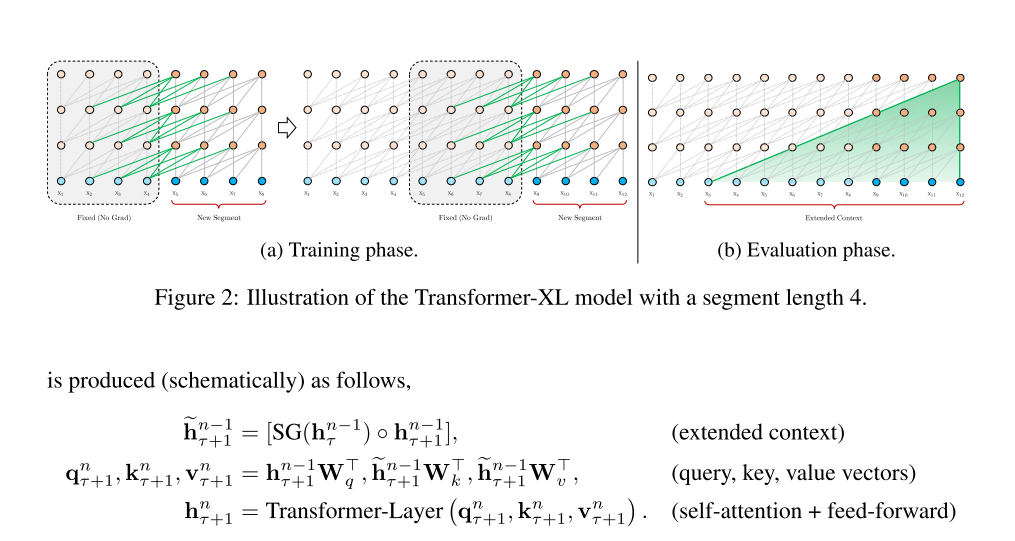
\includegraphics[scale=0.5]{images/transformerxl}
	\caption{\label{fig:transformerxl}Overview of transformer-xl which uses extended context to solve the problem of sending large sequences through Transformers.}
\end{figure*}

